\section{Analyse du marché et des besoins}
Afin de developper un produit qui puisse convenir aux besoins des personnes souffrant de begaiement ainsi qu'aux othopédistes, j'ai effectué quelques recherches pour définir les exercices utilisés par les orthopédistes pour aider leurs patients. Le projet devant être developpé en seulement 12 semaines, j'ai décidé de concentrer mes recherches uniquement en ligne sans démarcher de réelles orthopédistes qui m'auraient permis de cerner plus précisement les besoins réelles mais qui m'aurait aussi pris beaucoup plus de temps.

J'ai également fait une étude comparative des applications actuellement disponible sur le marché des application Android, un tableau récapitulatif est disponible dans l'annexe \ref{appendix:market}. Cette étude a relevé un manque d'application complète qui propose plusieurs exercices, les applications se concentrent souvent sur un seul exercice. Aussi, aucune application propose de faire le lien entre les bègues et leurs thérapistes.

Afin de décrire complétement le but de l'application, le contexte d'utilisation dans lequel elle s'inscit (\textit{par qui ? comment ? pourquoi ?}), ses fonctionnalités et autres diverses exigences (sécurité, maintenabilité, etc),  j'ai rédigé un \textit{Software Requirements Specification (SRS)}. Un \textit{SRS} est un document décrivant les exigences fonctionelles et non fonctionnelles, les intéractions de l'utilisateurs sur le produit et les eventuelles contraintes à respecter (lois et regulations, protocole à utiliser, limitations matériel, etc.). La table des matière de ce document est disponible dans l'annexe \ref{appendix:srs}. En particulier, ce document décrit précisemment les interaction de l'utilisateur sur l'application récapitulées dans le diagramme de cas d'utilisation de la figure \ref{fig:srs}. L'annexe \ref{appendix:srs_example} contient un exemple de spécification d'un cas d'utilisation.

\begin{figure}[h]
  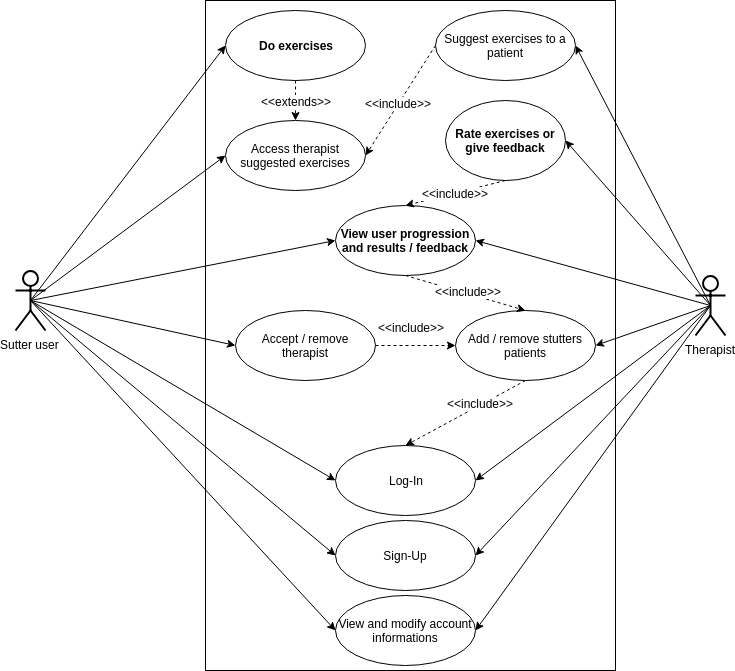
\includegraphics[width=.9\linewidth]{content/imgs/usecase.png}
  \caption{Diagramme cas d'utilisation}
  \label{fig:srs}
\end{figure}
